
%% bare_conf_compsoc.tex
%% V1.4b
%% 2015/08/26
%% by Michael Shell
%% See:
%% http://www.michaelshell.org/
%% for current contact information.
%%
%% This is a skeleton file demonstrating the use of IEEEtran.cls
%% (requires IEEEtran.cls version 1.8b or later) with an IEEE Computer
%% Society conference paper.
%%
%% Support sites:
%% http://www.michaelshell.org/tex/ieeetran/
%% http://www.ctan.org/pkg/ieeetran
%% and
%% http://www.ieee.org/

%%*************************************************************************
%% Legal Notice:
%% This code is offered as-is without any warranty either expressed or
%% implied; without even the implied warranty of MERCHANTABILITY or
%% FITNESS FOR A PARTICULAR PURPOSE! 
%% User assumes all risk.
%% In no event shall the IEEE or any contributor to this code be liable for
%% any damages or losses, including, but not limited to, incidental,
%% consequential, or any other damages, resulting from the use or misuse
%% of any information contained here.
%%
%% All comments are the opinions of their respective authors and are not
%% necessarily endorsed by the IEEE.
%%
%% This work is distributed under the LaTeX Project Public License (LPPL)
%% ( http://www.latex-project.org/ ) version 1.3, and may be freely used,
%% distributed and modified. A copy of the LPPL, version 1.3, is included
%% in the base LaTeX documentation of all distributions of LaTeX released
%% 2003/12/01 or later.
%% Retain all contribution notices and credits.
%% ** Modified files should be clearly indicated as such, including  **
%% ** renaming them and changing author support contact information. **
%%*************************************************************************


% *** Authors should verify (and, if needed, correct) their LaTeX system  ***
% *** with the testflow diagnostic prior to trusting their LaTeX platform ***
% *** with production work. The IEEE's font choices and paper sizes can   ***
% *** trigger bugs that do not appear when using other class files.       ***                          ***
% The testflow support page is at:
% http://www.michaelshell.org/tex/testflow/



\documentclass[9pt,conference]{IEEEtran}
% Some/most Computer Society conferences require the compsoc mode option,
% but others may want the standard conference format.
%
% If IEEEtran.cls has not been installed into the LaTeX system files,
% manually specify the path to it like:
% \documentclass[conference,compsoc]{../sty/IEEEtran}


\usepackage{float}
\usepackage{booktabs}


% Some very useful LaTeX packages include:
% (uncomment the ones you want to load)


% *** MISC UTILITY PACKAGES ***
%
%\usepackage{ifpdf}
% Heiko Oberdiek's ifpdf.sty is very useful if you need conditional
% compilation based on whether the output is pdf or dvi.
% usage:
% \ifpdf
%   % pdf code
% \else
%   % dvi code
% \fi
% The latest version of ifpdf.sty can be obtained from:
% http://www.ctan.org/pkg/ifpdf
% Also, note that IEEEtran.cls V1.7 and later provides a builtin
% \ifCLASSINFOpdf conditional that works the same way.
% When switching from latex to pdflatex and vice-versa, the compiler may
% have to be run twice to clear warning/error messages.






% *** CITATION PACKAGES ***
%
\ifCLASSOPTIONcompsoc
  % IEEE Computer Society needs nocompress option
  % requires cite.sty v4.0 or later (November 2003)
  \usepackage[nocompress]{cite}
\else
  % normal IEEE
  \usepackage{cite}
\fi
% cite.sty was written by Donald Arseneau
% V1.6 and later of IEEEtran pre-defines the format of the cite.sty package
% \cite{} output to follow that of the IEEE. Loading the cite package will
% result in citation numbers being automatically sorted and properly
% "compressed/ranged". e.g., [1], [9], [2], [7], [5], [6] without using
% cite.sty will become [1], [2], [5]--[7], [9] using cite.sty. cite.sty's
% \cite will automatically add leading space, if needed. Use cite.sty's
% noadjust option (cite.sty V3.8 and later) if you want to turn this off
% such as if a citation ever needs to be enclosed in parenthesis.
% cite.sty is already installed on most LaTeX systems. Be sure and use
% version 5.0 (2009-03-20) and later if using hyperref.sty.
% The latest version can be obtained at:
% http://www.ctan.org/pkg/cite
% The documentation is contained in the cite.sty file itself.
%
% Note that some packages require special options to format as the Computer
% Society requires. In particular, Computer Society  papers do not use
% compressed citation ranges as is done in typical IEEE papers
% (e.g., [1]-[4]). Instead, they list every citation separately in order
% (e.g., [1], [2], [3], [4]). To get the latter we need to load the cite
% package with the nocompress option which is supported by cite.sty v4.0
% and later.





% *** GRAPHICS RELATED PACKAGES ***
%
\ifCLASSINFOpdf
   \usepackage[pdftex]{graphicx}
  % declare the path(s) where your graphic files are
  % \graphicspath{{../pdf/}{../jpeg/}}
   \graphicspath{ {images/} }
  % and their extensions so you won't have to specify these with
  % every instance of \includegraphics
  % \DeclareGraphicsExtensions{.pdf,.jpeg,.png}
\else
  % or other class option (dvipsone, dvipdf, if not using dvips). graphicx
  % will default to the driver specified in the system graphics.cfg if no
  % driver is specified.
  % \usepackage[dvips]{graphicx}
  % declare the path(s) where your graphic files are
  % \graphicspath{{../eps/}}
  % and their extensions so you won't have to specify these with
  % every instance of \includegraphics
  % \DeclareGraphicsExtensions{.eps}
\fi
% graphicx was written by David Carlisle and Sebastian Rahtz. It is
% required if you want graphics, photos, etc. graphicx.sty is already
% installed on most LaTeX systems. The latest version and documentation
% can be obtained at: 
% http://www.ctan.org/pkg/graphicx
% Another good source of documentation is "Using Imported Graphics in
% LaTeX2e" by Keith Reckdahl which can be found at:
% http://www.ctan.org/pkg/epslatex
%
% latex, and pdflatex in dvi mode, support graphics in encapsulated
% postscript (.eps) format. pdflatex in pdf mode supports graphics
% in .pdf, .jpeg, .png and .mps (metapost) formats. Users should ensure
% that all non-photo figures use a vector format (.eps, .pdf, .mps) and
% not a bitmapped formats (.jpeg, .png). The IEEE frowns on bitmapped formats
% which can result in "jaggedy"/blurry rendering of lines and letters as
% well as large increases in file sizes.
%
% You can find documentation about the pdfTeX application at:
% http://www.tug.org/applications/pdftex





% *** MATH PACKAGES ***
%
\usepackage{amsmath}
% A popular package from the American Mathematical Society that provides
% many useful and powerful commands for dealing with mathematics.
%
% Note that the amsmath package sets \interdisplaylinepenalty to 10000
% thus preventing page breaks from occurring within multiline equations. Use:
%\interdisplaylinepenalty=2500
% after loading amsmath to restore such page breaks as IEEEtran.cls normally
% does. amsmath.sty is already installed on most LaTeX systems. The latest
% version and documentation can be obtained at:
% http://www.ctan.org/pkg/amsmath





% *** SPECIALIZED LIST PACKAGES ***
%
%\usepackage{algorithmic}
% algorithmic.sty was written by Peter Williams and Rogerio Brito.
% This package provides an algorithmic environment fo describing algorithms.
% You can use the algorithmic environment in-text or within a figure
% environment to provide for a floating algorithm. Do NOT use the algorithm
% floating environment provided by algorithm.sty (by the same authors) or
% algorithm2e.sty (by Christophe Fiorio) as the IEEE does not use dedicated
% algorithm float types and packages that provide these will not provide
% correct IEEE style captions. The latest version and documentation of
% algorithmic.sty can be obtained at:
% http://www.ctan.org/pkg/algorithms
% Also of interest may be the (relatively newer and more customizable)
% algorithmicx.sty package by Szasz Janos:
% http://www.ctan.org/pkg/algorithmicx




% *** ALIGNMENT PACKAGES ***
%
%\usepackage{array}
% Frank Mittelbach's and David Carlisle's array.sty patches and improves
% the standard LaTeX2e array and tabular environments to provide better
% appearance and additional user controls. As the default LaTeX2e table
% generation code is lacking to the point of almost being broken with
% respect to the quality of the end results, all users are strongly
% advised to use an enhanced (at the very least that provided by array.sty)
% set of table tools. array.sty is already installed on most systems. The
% latest version and documentation can be obtained at:
% http://www.ctan.org/pkg/array


% IEEEtran contains the IEEEeqnarray family of commands that can be used to
% generate multiline equations as well as matrices, tables, etc., of high
% quality.




% *** SUBFIGURE PACKAGES ***
%\ifCLASSOPTIONcompsoc
%  \usepackage[caption=false,font=footnotesize,labelfont=sf,textfont=sf]{subfig}
%\else
%  \usepackage[caption=false,font=footnotesize]{subfig}
%\fi
% subfig.sty, written by Steven Douglas Cochran, is the modern replacement
% for subfigure.sty, the latter of which is no longer maintained and is
% incompatible with some LaTeX packages including fixltx2e. However,
% subfig.sty requires and automatically loads Axel Sommerfeldt's caption.sty
% which will override IEEEtran.cls' handling of captions and this will result
% in non-IEEE style figure/table captions. To prevent this problem, be sure
% and invoke subfig.sty's "caption=false" package option (available since
% subfig.sty version 1.3, 2005/06/28) as this is will preserve IEEEtran.cls
% handling of captions.
% Note that the Computer Society format requires a sans serif font rather
% than the serif font used in traditional IEEE formatting and thus the need
% to invoke different subfig.sty package options depending on whether
% compsoc mode has been enabled.
%
% The latest version and documentation of subfig.sty can be obtained at:
% http://www.ctan.org/pkg/subfig




% *** FLOAT PACKAGES ***
%
%\usepackage{fixltx2e}
% fixltx2e, the successor to the earlier fix2col.sty, was written by
% Frank Mittelbach and David Carlisle. This package corrects a few problems
% in the LaTeX2e kernel, the most notable of which is that in current
% LaTeX2e releases, the ordering of single and double column floats is not
% guaranteed to be preserved. Thus, an unpatched LaTeX2e can allow a
% single column figure to be placed prior to an earlier double column
% figure.
% Be aware that LaTeX2e kernels dated 2015 and later have fixltx2e.sty's
% corrections already built into the system in which case a warning will
% be issued if an attempt is made to load fixltx2e.sty as it is no longer
% needed.
% The latest version and documentation can be found at:
% http://www.ctan.org/pkg/fixltx2e


%\usepackage{stfloats}
% stfloats.sty was written by Sigitas Tolusis. This package gives LaTeX2e
% the ability to do double column floats at the bottom of the page as well
% as the top. (e.g., "\begin{figure*}[!b]" is not normally possible in
% LaTeX2e). It also provides a command:
%\fnbelowfloat
% to enable the placement of footnotes below bottom floats (the standard
% LaTeX2e kernel puts them above bottom floats). This is an invasive package
% which rewrites many portions of the LaTeX2e float routines. It may not work
% with other packages that modify the LaTeX2e float routines. The latest
% version and documentation can be obtained at:
% http://www.ctan.org/pkg/stfloats
% Do not use the stfloats baselinefloat ability as the IEEE does not allow
% \baselineskip to stretch. Authors submitting work to the IEEE should note
% that the IEEE rarely uses double column equations and that authors should try
% to avoid such use. Do not be tempted to use the cuted.sty or midfloat.sty
% packages (also by Sigitas Tolusis) as the IEEE does not format its papers in
% such ways.
% Do not attempt to use stfloats with fixltx2e as they are incompatible.
% Instead, use Morten Hogholm'a dblfloatfix which combines the features
% of both fixltx2e and stfloats:
%
% \usepackage{dblfloatfix}
% The latest version can be found at:
% http://www.ctan.org/pkg/dblfloatfix




% *** PDF, URL AND HYPERLINK PACKAGES ***
%
\usepackage{url}
% url.sty was written by Donald Arseneau. It provides better support for
% handling and breaking URLs. url.sty is already installed on most LaTeX
% systems. The latest version and documentation can be obtained at:
% http://www.ctan.org/pkg/url
% Basically, \url{my_url_here}.




% *** Do not adjust lengths that control margins, column widths, etc. ***
% *** Do not use packages that alter fonts (such as pslatex).         ***
% There should be no need to do such things with IEEEtran.cls V1.6 and later.
% (Unless specifically asked to do so by the journal or conference you plan
% to submit to, of course. )


% correct bad hyphenation here
\hyphenation{op-tical net-works semi-conduc-tor}


\begin{document}
%
% paper title
% Titles are generally capitalized except for words such as a, an, and, as,
% at, but, by, for, in, nor, of, on, or, the, to and up, which are usually
% not capitalized unless they are the first or last word of the title.
% Linebreaks \\ can be used within to get better formatting as desired.
% Do not put math or special symbols in the title.
\title{Comparative Analysis of Phonetic Algorithms \\Applied to Spanish}


% author names and affiliations
% use a multiple column layout for up to three different
% affiliations
\author{
    \IEEEauthorblockN
    {
        Axel A. Garcia Fuentes$^{1}$,
        Irene Payan Parra$^{1}$,\\
        J. Ubaldo Quevedo-Torrero$^{2}$
        and Rogelio Davila Perez$^{1}$\\
        \\
    }
    \IEEEauthorblockA
    {
        $^{1}$Graduate Division in Computer Science\\
        Universidad Autonoma de Guadalajara\\
        Zapopan, Mexico\\
        axel.garcia@edu.uag.mx\\
        irene.payan.p@gmail.com\\ 
        rdav90@gmail.com\\
        \\
    }
    %\IEEEauthorblockN{Jesus Ubaldo Quevedo-Torrero}
    \IEEEauthorblockA
    {
        $^{2}$Computer Science Department\\
        University of Wisconsin Parkside\\
        Wisconsin, USA\\
        quevedo@uwp.edu
    }
}

% conference papers do not typically use \thanks and this command
% is locked out in conference mode. If really needed, such as for
% the acknowledgment of grants, issue a \IEEEoverridecommandlockouts
% after \documentclass

% for over three affiliations, or if they all won't fit within the width
% of the page, use this alternative format:
% 
%\author{\IEEEauthorblockN{Michael Shell\IEEEauthorrefmark{1},
%Homer Simpson\IEEEauthorrefmark{2},
%James Kirk\IEEEauthorrefmark{3}, 
%Montgomery Scott\IEEEauthorrefmark{3} and
%Eldon Tyrell\IEEEauthorrefmark{4}}
%\IEEEauthorblockA{\IEEEauthorrefmark{1}School of Electrical and Computer Engineering\\
%Georgia Institute of Technology,
%Atlanta, Georgia 30332--0250\\ Email: see http://www.michaelshell.org/contact.html}
%\IEEEauthorblockA{\IEEEauthorrefmark{2}Twentieth Century Fox, Springfield, USA\\
%Email: homer@thesimpsons.com}
%\IEEEauthorblockA{\IEEEauthorrefmark{3}Starfleet Academy, San Francisco, California 96678-2391\\
%Telephone: (800) 555--1212, Fax: (888) 555--1212}
%\IEEEauthorblockA{\IEEEauthorrefmark{4}Tyrell Inc., 123 Replicant Street, Los Angeles, California 90210--4321}}




% use for special paper notices
%\IEEEspecialpapernotice{(Invited Paper)}




% make the title area
\maketitle

% As a general rule, do not put math, special symbols or citations
% in the abstract
\begin{abstract}
Text mining is a field of interest. It may use as input text written in natural language
for which is error prone. However, some of the typographical errors made while
typing may be imperceptible at a glance by a human being. In spite of that assumption,
they may be sufficient to cause a failure when using a computer to search a record in 
a database or maybe when processing natural language corpora. Efforts have been
done in the past to make some computer programs more robust against typographical 
errors. The present work discusses what a phonetic algorithm is and it proposes a 
precision measurement method for phonetic algorithms. It presents the results of 
applying the underlined method on text written in Spanish using natural language.\\

\textit{Keywords}: Natural Language Processing, Spanish, Phonetic algorithm.\\

Submission for "Regular Research Papers"
\end{abstract}

% no keywords





% For peer review papers, you can put extra information on the cover
% page as needed:
% \ifCLASSOPTIONpeerreview
% \begin{center} \bfseries EDICS Category: 3-BBND \end{center}
% \fi
%
% For peerreview papers, this IEEEtran command inserts a page break and
% creates the second title. It will be ignored for other modes.
\IEEEpeerreviewmaketitle



%%*************************************************************************
\section{Introduction}
%%*************************************************************************
Recently in history there have been efforts on finding an algorithm capable
of encode the sound of a word. At the beginning of the 20\textsuperscript{th} century in USA 
those efforts were used as a resource during one of the census in that country\cite{ref:27}.
Given names from several places in the world had to be inputted and several of them
did not have a clear writing from for the data analysts. It is possible that situation 
caused typographic errors and most likely because of the homophony between several 
proper names; e.g. Smith and Schmit or Moskowitz and Moskovitz. They sound very similar 
to people, however, they represent a computational issue since they are not the 
same for a traditional computer system. Something had to be done in order 
to properly classify or to correctly index the names of all those people.\\

One of the first algorithms used when looking for a solution to that problem is called Soundex. It was 
developed by Robert Russell and Margaret Odell in 1918\cite{ref:28}\cite{ref:33}. A variation of that
algorithm called American Soundex was used in the US census of 1930\cite{ref:01}\cite{ref:02}\cite{ref:25}. 
% American Soundex was referred to as Miracode: http://west-penwith.org.uk/misc/soundex.htm
It was used during a while until a deficiency on handling foreign names was identified\cite{ref:08}
\cite{ref:32}\cite{ref:24}. After Soundex some variants were used; e.g. Daitch-Mokotoff Soundex\cite{ref:38},
NYIIS\cite{ref:29}, Metaphone\cite{ref:29}, Beider-Morse Phonetic Matching\cite{ref:30}, Koelner Phonetik, MRA, Caverphone\cite{ref:29}
and PhoneticSpanish\cite{ref:09} to mention some of them. Those algorithms 
were called phonetic algorithms since they generate a result based on the
assumed sound the letters may have when written together. More details 
about this type of algorithm will be discussed in the following sections.\\

Objective of those algorithms is to create a resulting code that represents
the sound that a given word may produce when it is pronounced. That means, 
for any arbitrary pair of words, if they share the same resulting code then they are
assumed to be homophones, i.e. they are pronounced exactly in the same way. 
The combination of the characters (letters) in the word will create the word sound 
when it is pronounced. In a similar way, the algorithm uses the letters that compose 
the word as input. Trying to mimic the effect they have in the word sound, it will use 
those letters interactions in order to create a resulting code which will be referred as 
phonetic code. \\

Nevertheless, even if homophones can be found that do not imply
they are homonyms. The fact that words sound the same is not enough to cause the
words to share the same meaning. There is a deep difference between sound and 
meaning. Thus, the focus of this discussion is how effective the studied phonetic 
algorithms are to represent the word being analyzed. This document will disregard its 
meaning, as well as, the actual sound of the word. \\
 
 
 

%%*************************************************************************
\section{Phonetic Algorithms}
%%*************************************************************************
The variety of names that have been given to the actual algorithms under discussion consider: 
name encoding algorithms\cite{ref:17}, 
phonetic algorithms\cite{ref:01} and phonetic coding algorithms\cite{ref:10}, 
to mention some of them. The former evoke the usage those algorithms had during the census 
of 1930 in USA. Notwithstanding, they can be used to process other words besides names. 
Last two names mention the concept of "phonetic". In linguistics there exist two major areas 
that study the sound of the words: i.e. phonetics and phonology. Both areas have different 
purposes\cite{ref:31}.

\subsection{Phonetic and Phonology}
In Linguistic they are two areas that study the sound of the language and the effect the 
sound has on the language itself. Those areas are phonetic and phonology\cite{ref:03}. 
Phonetics study the way in which pronunciation sounds are generated. For that purpose 
it uses acoustic analyses, as well as, analyses of what sounds are heard by the
human ear. It elaborates more on the way people articulates the sounds. It considers in those 
analyses the parts of the phonic apparatus: tongue, throat, vocal cords, palate, soft palate, 
alveolus, teeth and lips\cite{ref:06}\cite{ref:07}\cite{ref:18}.\\

According with\cite{ref:31} phonology studies elements called "phonemes". They are part of
the study of how the sounds affect the language. The following example is being taken from 
the same authors and it is being used to illustrate what phonology studies: 
In a language there exist a sound set for which varying a single aspect of them causes a
radical variation of its meaning. Example is the following, in the word \lbrack p{\'o}ka\rbrack
"poca" (which in english could be interpreted as "little" or "few") the first sound is a voiceless 
bilabial stop, \lbrack p\rbrack. If the vibration factor of the vocal cords varies when pronouncing
that consonant, i.e. they are caused to vibrate, then the voiceless bilabial stop becomes a 
voiced bilabial stop \lbrack b\rbrack. The result of that change is a completely different word: 
\lbrack b{\'o}ka\rbrack "boca" (mouth).\\

Linguistics call "phonemes" to those sounds that should be invariant in order to keep the word meaning. 
Phonology studies phonemes (among other language aspects). Phonemes vary in each language, 
i.e. there are different phonemes in English than there are phonemes in Spanish, which in turn are 
different to German, Japanese, and so on. Thus phonemes are language dependent\cite{ref:06}\cite{ref:07}\cite{ref:18}.\\

Phonemes may be considered the functional reference to compare the sound of two words 
in a given language. If there
 is a difference in the phonemes used, then there are two different words being 
compared and the ideal algorithm should produce different resulting codes. Thus what the
algorithm is doing is processing the word in a phonological level. That may be enough 
justification to name these algorithms "phonological algorithms" and to refer to their result
"phonological code". However,  since the name "phonetic algorithms" seems to have been 
widely used by now, this document will use "phonetic algorithms" and "phonetic codes" for 
the rest of the discussion. 

\subsection{Phonetic Algorithms as Hash Algorithms}
Something to have in mind is phonetic algorithms were originally created to index words by the sound 
they produce when pronounced\cite{ref:02}. Using that as base, (in Spanish) "coro" and "koro" should
share the same phonetic code, whereas, "coro" and "choro" should not.  \\

Phonetic codes are the result of executing phonetic algorithm on a word. They have been used
to create the index of a name in the mentioned census of 1930. That resembles the usage of a
hash function and in fact, phonetic codes have been informally referred to as "phonetic hash". 
There is a number of desirable characteristics that a hash function should meet\cite{ref:16}. 
Phonetic algorithms are in deed hash functions and the reasoning is the following:
\begin{itemize}
\item \textbf{Weak Collision Resistance.} For any given word, if its pronunciation significantly changes then the 
phonetic algorithm should generate a different phonetic code.\\
\item \textbf{Strong Collision Resistance.} Consider those algorithms have been designed to generate the same
phonetic code for words that share the same pronunciation. In that way words can be grouped by phonetic
code. Two words that sound different should have different phonetic codes. That means phonetic 
algorithms are designed for low collision.\\
\item \textbf{Oneway Property.} Phonetic algorithms will ignore characters that are irrelevant to phonetic code 
production. It is not possible to turn it into the initial word since there is not enough information in the 
phonetic code to do it.\\
\item \textbf{Performance.} Phonetic algorithms are deterministic. Some of them look the characters of the word
in a map/dictionary that contains the phonetic code transformation. Structures like maps or dictionaries use
to be O(n) where n is equals to the word length or less. Assuming that a word has a small number of 
characters, then their computation time is reasonable.\\
\end{itemize}


There are some phonetic algorithms that have been created. Some of them were designed to process text 
assuming an English context. Some others where extended to languages other than English. Next 
sections will discuss some of the phonetic algorithms that has been used in the past.\\
 
\begin{itemize}
\item \textbf{Soundex.}
It was used in 1930 during retrospective analysis of US census of 1890-1920\cite{ref:01}.  The initial 
version of the system was patented by Margaret Odell and Robert Russell in 1918 as U.S. Pat. No. 1,261,167\cite{ref:33}and 1,435,663 (1922)\cite{ref:34}.
It was used to index given names based on their pronunciation in English. Each Soundex code consist 
of a letter and three digits; e.g. W�252. The letter us the initial of the surname. The digits are assigned 
based on the subsequent letters in the surname. The objective is to build a code of four elements; 
zeros are padded as required\cite{ref:02}\cite{ref:24}.

The so-called "American Soundex" system is an improvement on Russell's invention, and was 
used by the National Archives and Record Administration to index the 1880, 1890, 1900, 1910, 
and 1920 U.S. Censuses\cite{ref:33}.

With some minor changes to the weighting scheme used, Soundex has been applied to languages 
other than English\cite{ref:34}\cite{ref:35}.\\

\item \textbf{Daitch-Mokotoff Soundex System.}
This variation of Soundex was Motivated by the poor results when dealing with Slavic and Yiddish 
surnames. Its creators were the jewish genealogist Gary Mokotoff and Ranndy Daitch from Jewish 
Genealogical Society. In 1985 Mokotoff indexed the names of 28,000 people that legally changed 
their names while living in Palestine during 1921 through 1948. The majority of them were Jewish 
with germanic or slavic names. During that exercise there were names that sounded the same. 
However, Soundex did not generate the same phonetic code; e.g. Moskowitz y Moskovitz\cite{ref:08}
\cite{ref:32}\cite{ref:24}.
	
The following examples were obtained from\cite{ref:39}:
\begin{table}[H]
\caption{Phonetic Algorithms: Ponetic codes Comparison} \label{tab:02}
\centering
\begin{tabular}{ lcp{0.35\columnwidth} }\\
\toprule[1.5pt]
                             & \multicolumn{2}{c}{\bf Generated Phonetic Codes of Phonetic Algorithms} \\
	\bf Surname & \bf American Soundex & \bf D-M Soundex \\ \hline
         Peters	&P362	&739400, 734000 \\
         Peterson	&P362	&739460, 734600 \\
         Moskowitz &M232	&645740 \\
         Moskovitz	 &M213	&645740 \\
         Auerbach	&A612	&097500, 097400 \\
         Uhrbach	&U612	&097500, 097400 \\
         Jackson	&J250	&154600, 454600, 145460, 445460 \\
         Jackson-Jackson	&J252	&154664, 454664,145466, 445466, 154646, 454646, 145464, 445464 \\
\bottomrule[1.25pt]
\end{tabular}
\label{default}
\end{table}%






\item \textbf{NYSIIS (New York State Identification and Intelligence System).}
Developed circa 1970 after several attempts to improve the Soundex algorithm. NYSIIS creates a 
string of up to six characters. See more details in \cite{ref:17}\cite{ref:24}.\\


\item \textbf{Metaphone.}
It was published in 1990 as an enhancement to Soundex. It was designed for English language.
This phonetic algorithm has been used to perform genealogical searches. There are versions of
this algorithm implemented for high level languages like: Pythoh and PHP to mention some\cite{ref:11}
\cite{ref:13}\cite{ref:22}\cite{ref:24}.\\


\item \textbf{Double-Metaphone.}
It was developed circa 2000. It is an improvement to Metaphone. It produces two phonetic codes 
for a single input word. The two phonetic codes are: the most likely pronunciation and the optimum 
pronunciation\cite{ref:17}\cite{ref:24}.\\


\item \textbf{Beider-Morse Phonetic Matching.} 
This algorithm considers that the pronunciation of a given word depends on the language
where that word is being pronounced. First step is to identify the word language. Then
the word is analyzed and broken down into phonetic tokens. That is performed by using
pronunciation rules for the detected language. Phonetic code is the sequence of phonetic
codes\cite{ref:19}\cite{ref:24}.\\


\item \textbf{PhoneticSpanish.}
This is a an algorithm proposed by\cite{ref:09} which is based on Soundex. The algorithm
tries to adapt Soundex to Spanish pronunciation. Authors does not mention any restriction
on the phonetic code length.\\
\end{itemize}



%%*************************************************************************
\section{Phonetic Algorithms Comparison Method}
%%*************************************************************************
\subsection{Precision Function}
\label{sec:PrecisionFunction} 
This section explains the shape of the mathematical function used to measure the studied
phonetic algorithm. \\

Each phonetic algorithm generates a phonetic code for a given word: $\phi(\alpha)=\alpha'$
It is possible that a a word could be associated to a distinct phonetic code depending on
the used phonetic algorithm:
\begin{multline}
% ??. ?1(?)=?1? , ?2(?)=?2? , ?3(?)=?3? ? ?1? =/ ?2? =/ ?3?
\exists\alpha.\ \ \phi_1(\alpha)=\alpha'_1,\phi_2(\alpha)=\alpha'_2,\phi_3(\alpha)=\alpha'_3 \land\ \\ \alpha'_1\ne\alpha'_2,\alpha'_2\ne\alpha'_3,\alpha'_3\ne\alpha'_1
\end{multline}

One of the goals of this comparison is to gather data that allows to measure how the studied
phonetic algorithms point to the correct word. In other words, how precise and accurate each
algorithm is. The following are the definitions of precision and accuracy considered for this
document:\\
\begin{itemize}
\item \textbf{Algorithm Precision.} Lets assume there are two words: "correct word" and a 
single "evaluation word". If the evaluation word were to be processed in order to find the 
correct word, then that processing requires one step to produce the result; i.e. processing 
the evaluation word will give as result the correct word. Now assume there are two
evaluation words and a single correct word. In that case, processing the result would 
require two steps; one for each evaluation word. If there were three evaluation words
then the evaluation would be three steps, and so on. Precision is how far the processing is
from the correct word. Which in few words mean, how many words share the same phonetic 
code given a phonetic algorithm. Paragraphs below explain that with more details.\\
\item \textbf{Algorithm Accuracy.} The evaluation word phonetic code matches the correct 
word phonetic code.\\
\end{itemize}

The name used in this document for the set of words that share the same phonetic code is 
"recommendation set". Each one of those words are considered a valid replacement alternative. 
Consider the following premises:
\begin{enumerate}
% 1
\item Based on the discussion about phonetics, the pronunciation of each one of the alternatives $\beta$
is equal to the pronunciation of the evaluation word $\alpha$. Thus, assumption is either of those $\beta$
could replace $\alpha$:
\begin{equation}
%????. p(?) = p(?) ? ? ? ?, ???????
\forall\alpha.\beta.\Theta.\left\{\ (\phi(\alpha) = \phi(\beta)) \to (\alpha=\beta\ \land\ \beta\in\Theta)\right\}
\end{equation}

% 2
\item However, only a single one of them can be part of the solution set $\Psi$; i.e. $\left\|\Psi\right\|$=TP=1. The rest of them are considered
false positives (FP):
\begin{multline}
\label{eq_01}
%????. ??? ???? ? |?| = 1
\forall\beta.\gamma.\Theta.\Psi.\{(\beta\in\Theta\land\gamma\in\Theta\land \gamma\ne\beta) \to\\ (\gamma\in\Psi\ \land\ \beta\notin\Psi\ \land\ \left\|\Psi\right\|=1)\}
\end{multline}

% 3
\item A False Negative (FN) is actually a True Positive (TP) incorrectly classified; i.e. $\neg$FN is TP. Based on (\ref{eq_01}), true positives set $\Psi$ has a single element $\gamma$. Thus, in this context FN and TP are considered the same:
\begin{equation}
%??. ~~ ? ? ?
\forall\gamma.\Psi.\{(\neg\neg\gamma\in\Psi\land\gamma\in\Psi\land\left\|\Psi\right\|=1)\to\neg\neg\gamma=\gamma\}
\end{equation}
\begin{equation}
TP+FN=1
\end{equation}

% 4
\item Phonetic codes are True Positives candidates. As (\ref{eq_01}) states there is a single one 
TP, the other $\beta$ candidates are a False Positives(FP), and they are represented by 
$\Delta$ set:
\begin{equation}
\label{eq_02}
\forall\beta.\gamma.\Delta.\ \{(\beta\in\Delta\land\gamma\notin\Delta) \to\left\|\Delta\right\|=N-1\}
\end{equation}
Where $N$ is the length of the alternatives set $\Theta$.
\begin{equation}
\left\|\Theta\right\|=N
\end{equation}

% 5
\item 
By definition phonetic codes are TP candidates. That means none of them is meant not to be
an alternative candidate and thus none of them is a True Negative(TN)
\begin{equation}
TN=0
\end{equation}

% 6
\item Accuracy equation has the following form:
\begin{equation}
accuracy=\frac{TP+ TN}{TP + FP + FN + TN}
\label{eq_03}
\end{equation}

Updating (\ref{eq_03}) with considerations of (\ref{eq_01}) and (\ref{eq_02}) precision equation has the following transformation:
\begin{multline}
accuracy=\frac{TP+ TN}{(TP + FN) + (TN+ FP)} \to \\ \frac{1+ 0}{1 + (N-1)} \to \frac{1}{N}
\label{eq_05}
\end{multline}


% 7
\item Precision equation has the following form:
\begin{equation}
precision=\frac{TP}{TP + FP}
\label{eq_04}
\end{equation}

Updating (\ref{eq_04}) with considerations of (\ref{eq_01}) and (\ref{eq_02}) precision equation has the following transformation:
\begin{equation}
precision=\frac{TP}{TP + FP} \to \frac{1}{1 + (N-1)} \to \frac{1}{N}
\label{eq_06}
\end{equation}


\end{enumerate}

Equations (\ref{eq_05}) and (\ref{eq_06}) have the same form. Thus a single 
equation can be used to measure both characteristics, i.e. precision and accuracy.
However, a result that does not contain the looked for result will not be considered
precise:
\[   
precision = 
     \begin{cases}
       \text{$\frac{1}{N}$}\quad\text{Correct word found}\\
       \text{$0$}\quad\text{Otherwise}\
     \end{cases}
\] 



%%*************************************************************************
\section{Method}
%%*************************************************************************
A sample of 1000 tweets was used for this experiment. Those tweets were gathered
without a particular constrain. The text in those tweets is natural language in Spanish
spoken in Mexico. That includes slang, words created by the tweet author, text 
emoticons, as well as, official Spanish words. The input data also has structured strings 
like: urls, numbers and hashtags to mention some.\\

It is important to mention that the language used in social networks is most likely informal.
The data presents words with alterations with respect their respective formal mode. Altered 
words are those which do not appear in the lexical resource(i.e. Spanish dictionary). 
Formal words are those contained in the lexical resource.

The following are identified cases of altered words and the approach used to handle those
cases:\\

\begin{itemize}
\item \textbf{Unnecessary repeated letters.}
For example "lentisssssssssimo" 
instead of "lent{\'i}simo" which could be interpreted as "extremely slow". Another occurrence 
of this same example is "Aaaaaaaaaaaah" instead of "ah" which is an interjection used to
express sorrow, exclamation, surprise or a similar feeling according with the Royal Spanish
Academy. In this example both words have an exact match in the Royal Spanish Academy
dictionary. For those cases, the word with unnecessary repeated letters was transformed
to its Royal Spanish Academy form.\\

\item \textbf{Incorrect Characters in a formal word.}
  For example "caf\v{Z}" instead of "caf{\'e}" (coffe), 
"con\v{Z}ctese" instead of "con{\'e}ctese" (interpreted as "make a connection to"), "T\=O\OE cnico"
instead of "T{\'e}cnico"("Technician"). In this example both words have an exact match in the 
Royal Spanish Academy dictionary, too. For those cases, the word with incorrect characters
has been transformed to its Royal Spanish Academy form.\\


\item \textbf{Ambiguous Words.}
For example: "T?pico" may be "T{\'o}pico"(topic) or "T{\'i}pico"(typic), "est?" may be
 "est{\'a}" or "est{\'e}" (to be). Correct term may be inferred from the context where the 
word is being used. However, it has been decided to ignore those words since finding the 
correct selection goes beyond the scope of phonetic algorithms. Doing such search may 
introduce systematic errors in the measurements of this experiment.\\
\end{itemize}
 
The above described control mechanism has been used in order to prevent systematic 
errors on the data given that fact is to Tweet author decides to ignore orthography rules.\\

A Python script was used for this evaluation. That evaluation script uses a non-standard 
dictionary of terms. That Spanish dictionary of terms gathers words written in Spanish
which were collected from several public resources. That made it useful for this work.
Evaluation is divided in the following stages:\\

\begin{itemize}
\item Phonetic Code Generation. Dictionary of terms was processed with each one of
the discussed algorithms. That generated a phonetic code for each one of the terms in
the dictionary. Phonetic codes were added into the dictionary of terms. The result is
the phonetic codes dictionary. \\

\item Precision Data Generation. For each one of the sample tweets, each one of the 
words in the tweet was searched in the dictionary of terms. Some words were found 
and some were not. The not found words were processed with the phonetic algorithm.
Their phonetic code was computed, associated to the not-found term and stored in a
different data resource for later use. That means, only the not-found terms were used
for the phonetic algorithm precision measurement. It was decided that way in order to
have a meaningful comparison; since terms found in the dictionary of terms are 
correctly formed by definition.\\
Data generated by this processing was saved in a comma-separated values file (cvs).
Each row in that file has the data generated by the processing done for a single word.
In other words, if a single tweet has several not-found words then there will be multiple
rows for that single tweet. The output CSV file is referred to as output map.\\

\item Results Generation. Comparison function mentioned in section \ref{sec:PrecisionFunction} 
was used in this stage. 

\end{itemize}

Algorithms execution time was not considered. Focus is the precision and accuracy of
the studied phonetic algorithms.


\section{Results}
The data samples in this section are not completely shown since the size of the results 
makes including the entire set unpractical. However, the full results set can be accessed
in unpublished \cite{ref:40}


Figure \ref{fig:preprocessed_tweet} shows a fragment of a CSV(comma separated 
value) file. The figure shows a portion of the sample of 1,000 tweets in Spanish.
\begin{figure}[H]
    \centering
    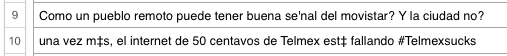
\includegraphics[width=\columnwidth]{results_01_20161024}
    \caption{Pre-processed tweet sample.}
    \label{fig:preprocessed_tweet}
\end{figure}

After the Python script processes the input data(see Fig. \ref{fig:preprocessed_tweet}) it 
generates as output another CSV file with the result data(see Fig. \ref{fig:processed_tweet}).
In the output data, the "Message ID" column is the identifier of the words of each tweet, 
"Item Name" column is the word that was analyzed, "Phonetic Code" is the phonetic 
code that was assigned to the word being processed, "Alternatives to Item" column are 
words that look similar to the word sound that was analyzed, "phonetic Algorithm precision" 
column is the precision computed using the method described in this document.
\begin{figure}[H]
    \centering
    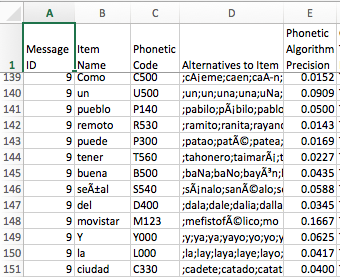
\includegraphics[width=0.8\columnwidth]{results_02_20161024}
    \caption{Processed tweet sample.}
    \label{fig:processed_tweet}
\end{figure}

At the right of Fig. \ref{fig:preprocessed_tweet} it is possible to see the "Message ID". For
instance, first row shows Message ID 9. In Fig. \ref{fig:processed_tweet}, the same Message
ID can be found. The resulting phonetic code of some of the words in that message
are shown. \\


Table \ref{tab:01} shows the studied phonetic algorithms ascendantly ordered by mean
as first criteria and then by median. That is, the lower in the table the algorithm is the
better precision it has.

\begin{table}[H]
\caption{Phonetic Algorithms Precision, Ascendent by Mean} \label{tab:01}
\centering
%\begin{center}
\centering
\begin{tabular}{ lccccc }\\
\toprule[1.5pt]
	\bf Algorithm & \bf Mean & \bf Median & \bf Std Dev \\ \hline
         Phonex	&0.0010	&0.0008	&0.0006\\
         Fuzzy Soundex	&0.0081	&0.0058	&0.0071\\
         Rusell Index	&0.0164	&0.0115	&0.0140\\
         Phonix	&0.0169	&0.0129	&0.0129\\
         Alpha Sis	&0.0191	&0.0143	&0.0161\\
         Soundex	&0.0202	&0.0165	&0.0137\\
         Double Metaphone	&0.0224	&0.0178	&0.0179\\
         Phonetik	&0.0253	&0.0183	&0.0207\\
         Sfinixbis	&0.0278	&0.0243	&0.0165\\
         Caverphone	&0.0317	&0.0252	&0.0235\\
         MRA	&0.0416	&0.0374	&0.0243\\
         Metaphone	&0.0464	&0.0416	&0.0287\\
         BMPM	&0.0532	&0.0497	&0.0302\\
         NYSIIS	&0.0536	&0.0474	&0.0318\\
         Phonet	&0.0838	&0.0803	&0.0355\\
         Phonem	&0.1036	&0.1011	&0.0444\\
\bottomrule[1.25pt]
\end{tabular}
%\end{center}
\label{default}
\end{table}%



%%*************************************************************************
\section{Conclusions and Future Work}
%%*************************************************************************
Used Spanish dictionary of terms has a mixture of official and non-official Spanish words, 
meaning the Royal Spanish Academy(Spanish: Real Academia Espa\~nola) does not 
recognize some of them. However, that is considered a positive aspect for this 
experiment because in the case of a misspelling that kind of words(i.e. non-official words)
are most likely to occur in natural language processing. Nevertheless, risk of a bias in the
manual labeling exist. That risk has been mitigated with a big sample size and the
re-usage of the same labeled dictionary for all of the phonetic algorithms evaluations.\\

Phonem and Phonet are the two algorithms with the highest precision mean among 
the studied phonetic algorithms in this work. Nevertheless, their precision is barely 
10\% which is distant from a promising precision. Future work should be done in order 
to find a phonetic algorithm capable of achieving a higher precision without using 
language context information.\\




%
% ---- Bibliography ----
%

\bibliographystyle{abbrv}
\bibliography{biblio}


\end{document}

